\documentclass[a4paper]{article}

\usepackage[english]{babel}
\usepackage[utf8]{inputenc}
\usepackage{amsmath}
\usepackage{graphicx}
\usepackage{listings}
\usepackage[colorinlistoftodos]{todonotes}
\title{Emergent Architecture Design}
\usepackage{authblk}

\author[1]{Boudewijn van Groos}
\author[2]{Chris Langhout}
\author[3]{Jens Langerak}
\author[4]{Paul van Wijk}
\author[5]{Louis Gosschalk}

\affil[1]{bvangroos \\
4229843}
\affil[2]{clanghout \\
4281705}
\affil[3]{jlangerak \\
4317327}
\affil[4]{pjvanwijk \\
4285034}
\affil[5]{lgosschalk \\
4214528}

\date{\today}

\begin{document}
\maketitle
\tableofcontents
\newpage

\section{Introduction}
This document describes the design of the architecture and it is continuously updated to the current state of the software. It also states the design goals we want to achieve during the project. Furthermore the subsystem decomposition is laid out.

\section{Design goals}
\subsection{Modularity}
The program can be split into a number of modules. These modules should be implemented independently of the other modules. Interaction between modules is only possible by making use of defined interfaces.

\subsection{Continuous Integration}
There should be always a working product. Each sprint should add one or more features.

\subsection{Understandability}
We must also make the software user-friendly. Even though the users of the
product are already familiar with analysis software, our application should be
easy to learn. It is essential that the user understands the usage of the
scripting language in our application before he/she is able to use it for
analysis.

\subsection{Code quality}
In the project we strive to have good code readability and the code must be easy to understand. This is also an important part of the static analysis. We handle the pull based system on Github. For each new feature that will be implemented the author of that feature must create a new branch and do all his work in that branch so that the master branch always consists of a working version of the software. If someone wants to commit he has to make a pull request first. His code will then be reviewed by at least 2 teammembers and eventually fixed before it can be merged with the working version in the master branch.\\
To improve code quality we have code conventions which the writer should follow before
his code is accepted. This is done by the Checkstyle plugin in the IDE that makes
sure these conventions are followed.


\section{Software architecture views}
\subsection{Subsystem decomposition}

\begin{figure}[h]
	\centering
    	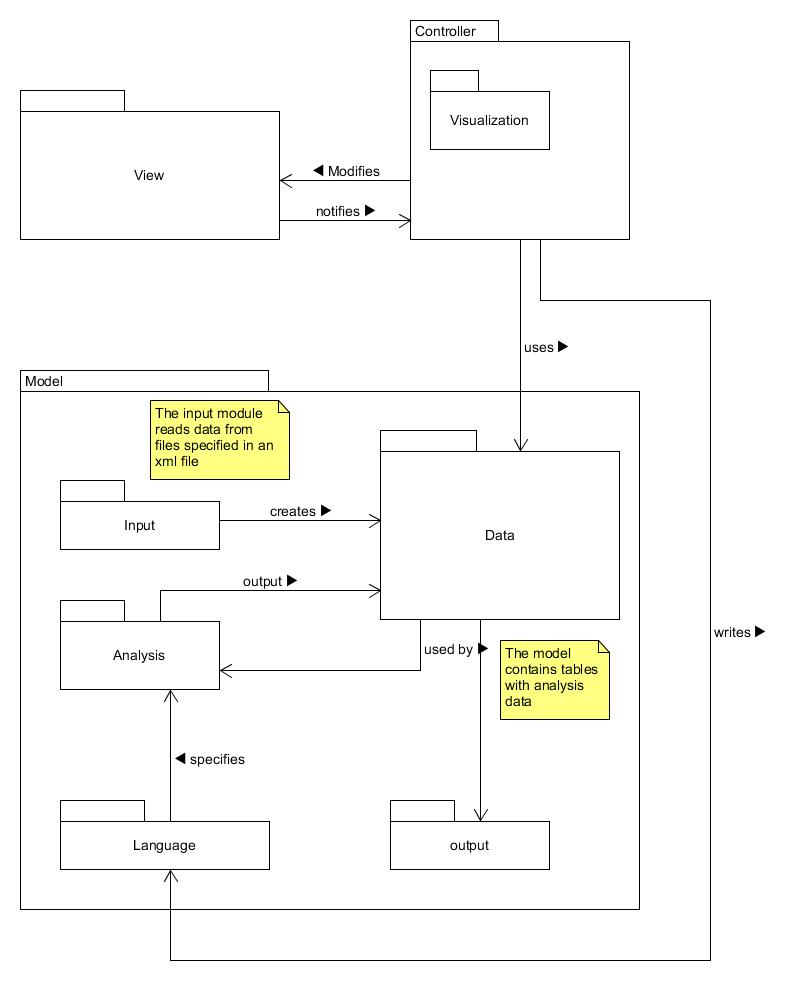
\includegraphics[scale=0.5]{images/modules.jpg}
    \caption{Modules of the system}
	\label{fig:modules}
\end{figure}

The input module should be able to read the data. With that data a dataModel
can be constructed. \\
The Analysis Specification module processes the script that defines how the
data should be analyzed. The user provides this script. This module translate
the script in operations that can be performed by the Analysis Module.\\
The Analysis Module perform the analyses over the dataModel. The output of this
module is the result of the analysis, this is a dataModel.\\
The Visualization module creates a certain visual representation of a
dataModel. For example it can create a box-plot of the creatine levels.

\subsection{State diagram}
Below is the state diagram which describes the flow of the program.
\begin{figure}[h]
	\centering
	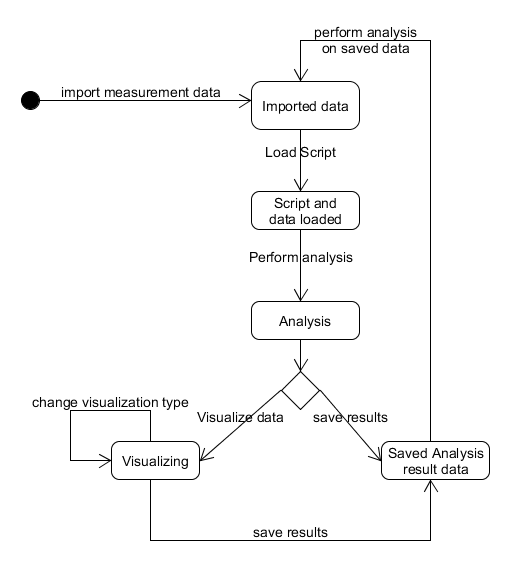
\includegraphics[scale=0.5]{images/statemachine.png}
	\caption{State diagram of the program}
	\label{fig:statemachine}
\end{figure}

\newpage

\section{Software architecture}

\subsection{Programming languages and auxiliary programs}
The software will mainly be written in Java since this was obligatory in
the project. For the graphical user interface we make use of the JavaFX
framework and is written using fxml. We use Eclipse and IntelliJ IDEA as IDE to
write the Java code with. 
For continuous integration and version control we use Git and Github. Locally we use Maven to build the project. On GitHub we use Travis CI to verify the builds.
We also use the JavaFX Scene Builder as a tool to design parts of the GUI because this provides a better preview of what the interface will look like while creating it.

\subsection{Used libraries}
\begin{description}
\item[JavaFX] Creating the graphical user interface.
\item[Mockito] Mocking objects to test behavior.
\item[Apache POI] Reading data analysis files stored in the Microsoft Excel format.
\item[Java SAX] Reading the xml file that specify the datafiles.
\end{description}

\section{Testing}
\subsection{Unit testing}
To make sure that all the code works as it should, the author must always write
unit tests for the code he has written. We make use of the JUnit framework to
write the tests. To verify behaviour of methods we use the Mockito framework to
stub certain object needed by the method.

\section{Glossarium}

\begin{description}

\item[Analysis] An analysis that can be done on measuring data to come to an answer to a specific question.

\item[Git \& GitHub] Git is the tool to control the versions in a repository. GitHub is the web-tool to make the versions available for group use.

\item[SUGAR] The scripting language used to create analyses.

\item[Pull Request] Are made on GitHub to get your commits to the code verified and merged with the master branch.

\end{description}

\end{document}
